%************************************************
\chapter{Theoretical background}
\label{ch:theoretical_bakcground}
%************************************************
In this chapter I will review the most important parts of the theory
of planetary dynamics. \Cref{sec:two_body} describes the two--body problem which 
introduces planet orbits and orbital elements. In \cref{sec:hamiltonian_mechanics}
I review the basic theory of a different formulation of mechanics called
\emph{Hamiltonian mechanics}. The Hamiltonian formalism and its tools will
be necessary for the development of an analytical model of resonance
capture in \cref{ch:analytical_model_of_high_order_mmrs}. In \cref{ch:pendulum}
I describe a useful toy model for studying mean--motion resonances -- the pendulum.
Finally, in \cref{ch:three_body} I review the theory of the three--body problem 
which forms the basis for subsequent chapters.

The second chapter deals with analytic models of mean--motion resonances
(MMRs for short). This concept is the key part of the thesis because the overlap
of MMRs and the passage of planetary or stellar bodies through them 
are crucial for the determination of the stability of planetary bodies. 
Here I develop a new analytical model of a 6:1 resonance in the case 
where the inner two bodies are 
comparable in mass. The 6:1 MMR is the first important resonance encountered
by circumbinary planets similar to the observed MS population once the 
binary starts evolving off the main--sequence. I use this 
model to predict the eccentricity kick to a planet orbiting the evolving
binary as the stars approach each other due to tidal forces. 

\section{The two--body problem}
\label{sec:two_body}
\subsection{The orbit equation and its solution}
If we are to attack the problem of three gravitionally interacting
bodies in a circumbinary system, we first need to understand a simpler 
problem -- that of two massive bodies. This problem is often called 
the \emph{Kepler problem}. Consider two bodies with masses
$m_1$ and $m_2$ and position vectors\footnote{Throughout the thesis,
vector quantities will be written with a bold--face font}
$\vect{r}_1$ and $\vect{r}_2$ relative to a fixed origin $O$ in
inertial space. The forces acting on the two bodies are given by
\begin{align}
    \vect{F}_1 &= Gm_1m_2 \frac{\vect{\hat{r}}}{r^3} = m_1\ddot{\vect{r}}_1\\
    \vect{F}_2 &= -Gm_1m_2 \frac{\vect{\hat{r}}}{r^3}= m_2\ddot{\vect{r}}_2
\end{align}
where $G=\SI{6.672}{\meter^3.kg^{-1}.s^{-2}}$ is the gravitational constant,
$\vect{\hat{r}}$ is the unit vector pointing from $\vect{r}_1$ to $\vect{r}_2$
and $r$ is the magnitude of the relative seperation vector 
$\vect{r}=\vect{r}_2 - \vect{r}_1$.
The double dots denote second time derivatives. From the definition of $\vect{r}$ 
and the equations of motion, it follows that
\begin{equation}
    \ddot{\vect{r}}=\ddot{\vect{r}}_2 - \ddot{\vect{r}}_1=-G(m_1+m_2)
    \frac{\vect{\hat{r}}}{r^3} \\
\end{equation}
which can be rewritten as
\begin{equation}
    \ddot{\vect{r}} + \mu \frac{\vect{\hat{r}}}{r^3} =0 \label{eq:4}
\end{equation}
where $\mu=G(m_1+m_2)$. If we take a cross product of \cref{eq:4} with
$\vect{r}\times$ from the left-hand side and using the fact that 
$\vect{r}\times\vect{r}=0$, we obtain
\begin{equation}
\vect{r}\times\ddot{\vect{r}}=0
\end{equation}
This can be integrated to get
\begin{equation}
    \vect{r}\times\dot{\vect{r}}=\vect{h}
    \label{eq:6}
\end{equation}
where $\vect{h}$ is a constant vector perpendicular to the plane spanned 
by $\vect{r}\times\dot{\vect{r}}$. $\vect{h}$ is in fact the angular momentum
per unit mass. Thus, the motion of $m_2$
relative to $m_1$ is confined to a plane perpendicular to $\vect{h}$. Since 
the motion is in a plane, we can simplify the problem further by transfering
to polar coordinated $(r,\theta)$ centered at $m_1$, we then have the following
relations between vectors available in any vector calculus book
\begin{align}
\vect{r} &=r\vect{\hat{r}}\\
    \dot{\vect{r}} &= \dot{r}\vect{\hat{r}} + r\dot{\theta}\boldsymbol{\hat\theta}\\
    \ddot{\vect{r}} &= (\dot{r} - r\dot{\theta}^2)\vect{\hat{r}} + \frac{1}{r} 
    \frac{d}{dt}\left(r^2\dot{\theta}\right)\boldsymbol{\hat\theta}\label{eq:9}
\end{align}
By substituting these transformations into \cref{eq:6} we get
\begin{equation}
\vect{h}=r^2\dot{\theta}\boldsymbol{\hat z}
    \label{eq:10}
\end{equation}
where $\boldsymbol{\hat z}$ is perpendicular to the orbital plane. 

By inserting the expression for $\ddot{\vect{r}}$ (\cref{eq:9}) into \cref{eq:4} 
and considering only the $\vect{\hat\r}$ component (the $\boldsymbol{\hat\theta}$
component just says that $h$ is constant which we know already), we have the following
scalar equation
\begin{equation}
\ddot{r}-r\dot{\theta}^2 + \frac{\mu}{r^2} =0
\end{equation}
To solve this differential equation, we use the substitution $r=u^{-1}$ and
\cref{eq:10}. From the chain rule, it follows
\begin{align}
    \dot{r}&=-h \frac{du}{d\theta} \\
    \ddot{r}&=-h^2u^2 \frac{d^2u}{d\theta^2} 
\end{align}
And finally, we have
\begin{equation}
    \frac{d^2u}{d\theta^2} +u= \frac{\mu}{h^2} 
    \label{eq:orbit_eq}
\end{equation}
\Cref{eq:orbit_eq} is called the \emph{orbit equation}. This second order 
differential equation has the solution (after transforming back to $r$)
\begin{equation}
    r = \frac{h^2/\mu}{1 + e\cos (\theta-\omega)} 
    \label{eq:orbit_eq_solution}
\end{equation}
where the \emph{eccentricity} $e$ and the \emph{argument of pericentre} $\omega$
are the two constants of integration. \Cref{eq:orbit_eq_solution} defines 
a \emph{conic section} curve in 2D space. Depending on the eccentricity,
it can either be an ellipse for $e<1$ corresponding to a closed orbit, or
a hyperbola for $e>1$ corresponding to an unbound orbit. The special case
$e=1$ defines a parabola but is of little physical significance since any
particular orbit is highly unlikely to have eccentricity exactly zero. 
Similarly $e=0$ defines a circular orbit which is of more interest since
most stable planetary orbits are very nearly circular.
\begin{figure}[htb]
\centering
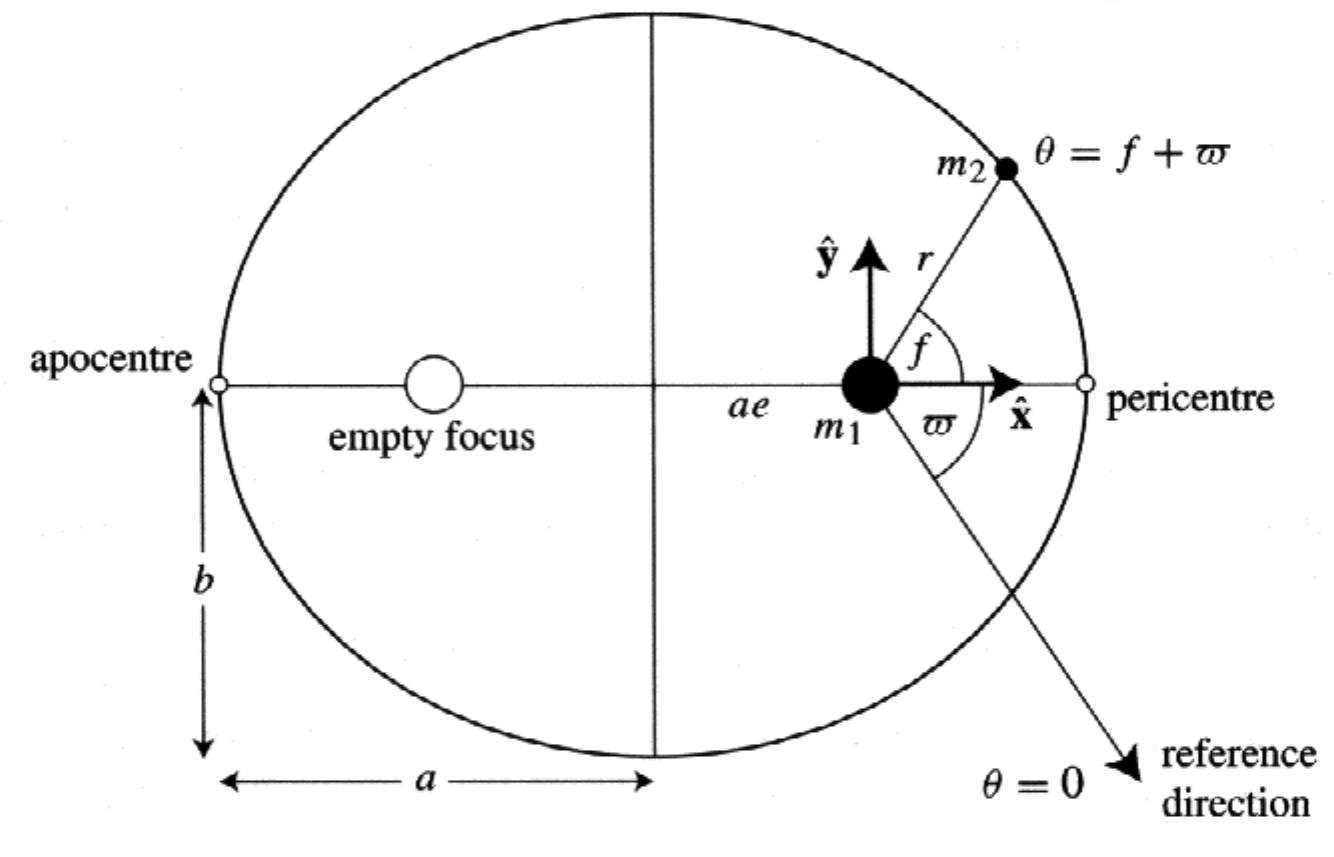
\includegraphics[width=\linewidth]{gfx/ellipse.png}
\caption{An elliptical orbit. The mass $m_1$ sits in one focus and $m_2$ orbits 
    around it. The postion of $m_2$ on the ellipse is specified by two angles, 
    the true anomaly $f$ and the argument of pericentre $\omega$. Only the $f$ 
    varies in the two--body problem, $\omega$ stays fixed in the absence of an
    external perturbation. Figure taken from \citeauthor{murray}.}
\label{fig:ellipse}
\end{figure}
\Cref{fig:ellipse} shows an elliptical orbit in two dimensional space. The mass
$m_2$ orbits around $m_1$ which is located in one of the focci of the ellipse.
The position of $m_2$ at each moment in time is described by the $2\pi$-periodic
angle 
$f=\theta - omega$ called the \emph{true anomaly}. The angle $\omega$ is specified 
relative to an arbitrary reference direction and it is constant throughout the 
motion. $f=0$ corresponds to the closest approach of $m_2$ to $m_1$, this point on
orbit is called the \emph{pericentre}. Conversely, the point furthest away from 
$m_2$ at $f=\pi$ is called the \emph{apocentre} . 
The \emph{semi-major axis} of the ellipse $a$ is given by
\begin{equation}
    a= \frac{h^2}{\mu} \frac{1+e}{1-e} 
\end{equation}
One can easily derive (\cite[ex.]{murray}) \emph{Kepler's third law} which says 
that
\begin{equation}
    T^2= \frac{4\pi^2}{\mu} a^3
    \label{eq:kepler_law}
\end{equation}
where $T$ is the orbital period of $m_2$ around $m_1$. We also define the so-called
\emph{mean motion} $n$, as
\begin{equation}
    n= \frac{2\pi}{T} 
\end{equation}
The mean motion is the average angular frequency of the periodic motion. It is 
constant in the two--body problem but in general varies when additional bodies are 
present.

If we multiply \cref{eq:4} by $\dot{\vect{r}}$ and use the expressions for
$\dot{\vect{r}}$ and $\ddot{\vect{r}}$ from \cref{eq:9}, we obtain the following
constant of motion
\begin{equation}
    \frac{1}{2} v^2 - \frac{\mu}{r} =C
\end{equation}
where $v^2=\dot{\vect{r}}\cdot\dot{\vect{r}}$ is velocity squared and $C$ is a
constant of motion, the energy per unit mass. It can be shown \citep{murray}
that $C$ is given by
\begin{equation}
    C= -\frac{\mu}{2a} 
\end{equation}
thus, of a closed orbit in the two--body problem depends only on the semi-major axis.
\subsection{The mean and eccentric anomaly}
By solving the orbit equation, we have established that the mass $m_2$ orbits 
around $m_1$ in an ellipse if $e<1$. However, it is not immediately clear how
to explicitly solve for the time dependance of $r$ and $f$ and thus determine 
the position of $m_2$ at any given time. It is obvious that $f$ and $r$ vary
non-linearly with time for $e\neq 0$. For reasons which will become apparent 
later, we would like to construct an angle which varies linearly with time.
One such angle is the \emph{mean anomaly} $M$ defined as
\begin{equation}
    M=n(t-\tau)
\label{eq:mean_anomaly}
\end{equation}
where $\tau$ is the \emph{time of pericentre passage} and is constant. $M$
incrases linearly with time at a rate equal to the mean motion. At $t=\tau$ 
we have $M=f=0$
and at $t=\tau + \T/2$ $M=f=\pi$, thus at the pericentre and apocentre 
M matches with $f$. The angle $M$ has no obvious geometricall significance
but we can define another angle which does. \Cref{fig:eccentric_anomaly} 
shows the orbital ellipse with semi-major axis $a$ together with a 
circumscribed circle of radius $a$ concentric with the ellipse. A line 
perpendicular to the semi-major axis of the ellipse interesects two points,
one on the orbit and one on the circumscribed circle. We define the 
\emph{eccentric anomaly} $E$ to be the angle between the semi-major axis
of the ellipse and the intersected point on the circle. Again, we have
$E=M=0$ at $f=0$ and $E=M=\pi$ at $f=\pi$. 
\begin{figure}[htb]
\centering
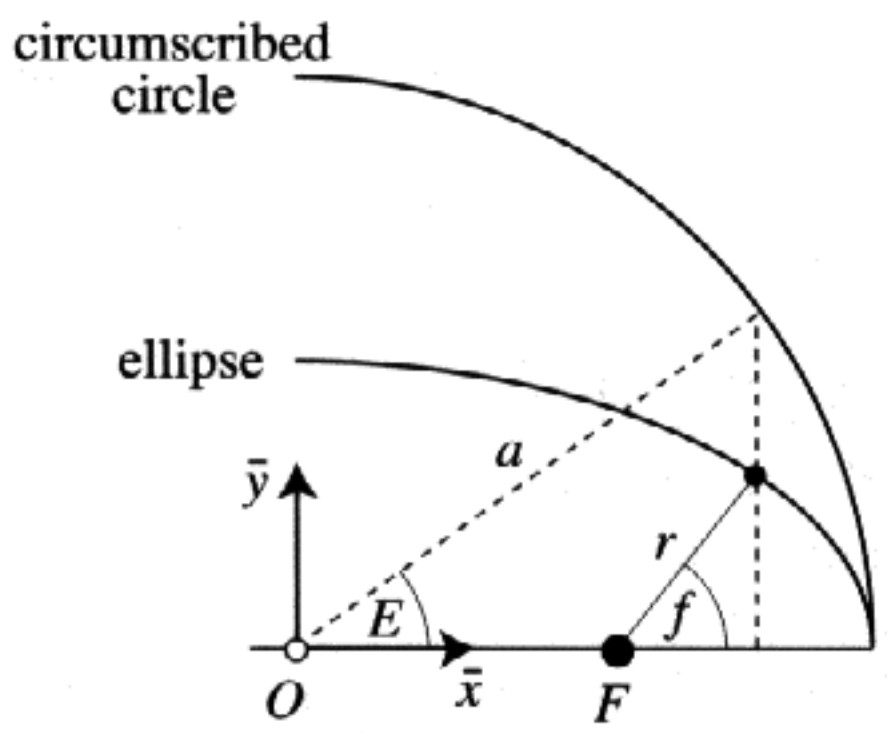
\includegraphics[width=0.5\linewidth]{gfx/eccentric_anomaly.png}
\caption{A geometrical description of the eccentric anomaly $E$.}
\label{fig:eccentric_anomaly}
\end{figure}
From geometry one can show that the following relation between the
angles $f$ and $E$ is satisfied
\begin{equation}
    \cos f= \frac{\cos E -e}{1-e\cos E} 
    \label{eq:eccentric_anomaly}
\end{equation}
Thus, there is a one-to-one correspondance between $f$ and $E$. To 
locate the location of the body on its orbit at time $t$, we need
a relationship between $E$ and $M$. This relation ship is called
the \emph{Kepler's equation} and is given by \citep{murray}
\begin{equation}
    M=E-e\sin E
    \label{eq:kepler_equation}
\end{equation}
A solution to this equation enables us to locate the body on its orbit
at any given time. The procedure is as follows
\begin{enumerate}
    \item At a particular time $t$ find $M$ from \cref{eq:mean_anomaly}
    \item Solve the Kepler's equation for $E$
    \item Use \cref{eq:eccentric_anomaly} to find $f$
\end{enumerate}
Kepler's equation is transcendental in $E$ and therefore it cannot
be solved directly. 

Finally, we define one last angle $\lambda$ called the
\emph{mean longitude} as
\begin{equation}
    \lambda =M +\omega
\end{equation}
Since it is derived from $M$, it does not have a geometrical 
interpretation. All longitudes are defined with respect to a 
common, arbitrary reference point.
\subsection{Orbit in an inertial frame}
So far we have derived a solution for the \emph{relative} motion
of $m_2$ with respect to $m_1$, we now turn to the description of the
orbit in a non-accelerating \emph{inertial frame}.
\begin{figure}[htb]
\centering
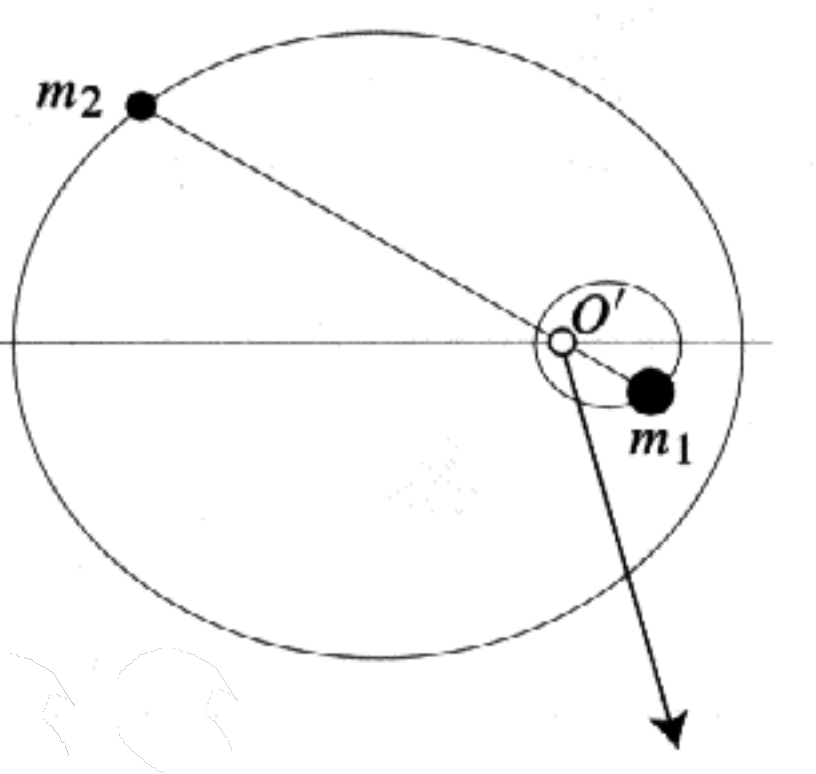
\includegraphics[width=0.5\linewidth]{gfx/barycentric_orbit.png}
\caption{The motion of $m_2$ and $m_1$ with respect to their centre
    of mass $O'$.}
\label{fig:barycentric_orbit}
\end{figure}
It is not difficult to show that the the masses $m_1$ and $m_2$ again
orbit in a conic section around their centre of mass with the same
period $T$ as before. 
\Cref{fig:barycentric_orbit} shows the orbits with respect to the
centre of mass. We need not worry about the motion of the centre
of mass itself because of a result from elementary mechanics which says
that the centre of mass of a collection of particles always moves at
constant velocity in a straight line and is therefore a valid inertial
reference frame. The conic sections of the orbits relative to the centre
of mass are 
reduced in scale by mass factors, as follows
\begin{equation}
    a_1= \frac{m_2}{m_1 + m_2} a\quad a_2= \frac{m_1}{m_1 + m_2} a
\end{equation}
where $a_1$ is the semi-major axis of the orbit of $m_1$ around $O'$
and $a_2$ is the semi-major axis of the orbit of $m_2$ around $O'$.

The \emph{total} angular momentum of the system is given by 
\begin{equation}
    L= \frac{m_1 m_2}{m_1 + m_2} \sqrt{\mu a(1-e^2)}
    \label{eq:ang_momentum}
\end{equation}
and the total orbital energy is
\begin{equation}
    E= -G \frac{m_1 m_2}{2a} 
\end{equation}
The energy of a Keplerian orbit depends only on the semi-major axis
and the angular momentum depends on both the semi-major axis and
the eccentricity. In particular, if the semi-major axis is constant
the only way to change the eccentricity is by changing the angular
momentum. This simple fact is the essence of so-called secular
interactions described in \cref{sec:three_body}. The angular momentum
is largest for a circular orbit.

\subsection{Orbit in three-dimensional space}
We have determined that the bodies in the two--body problem move on
on an ellipse in inertial space. The orientation of that ellipse 
stays fixed for all time if no external bodies are present. If there 
are also other bodies in the system however, the orbit no longer stays
fixed, both its shape and orientation change in three-dimensional space.
Because of that it is useful to define the orientation of the orbit
in 3D space relative to a fixed reference plane.
\begin{figure}[htb]
\centering
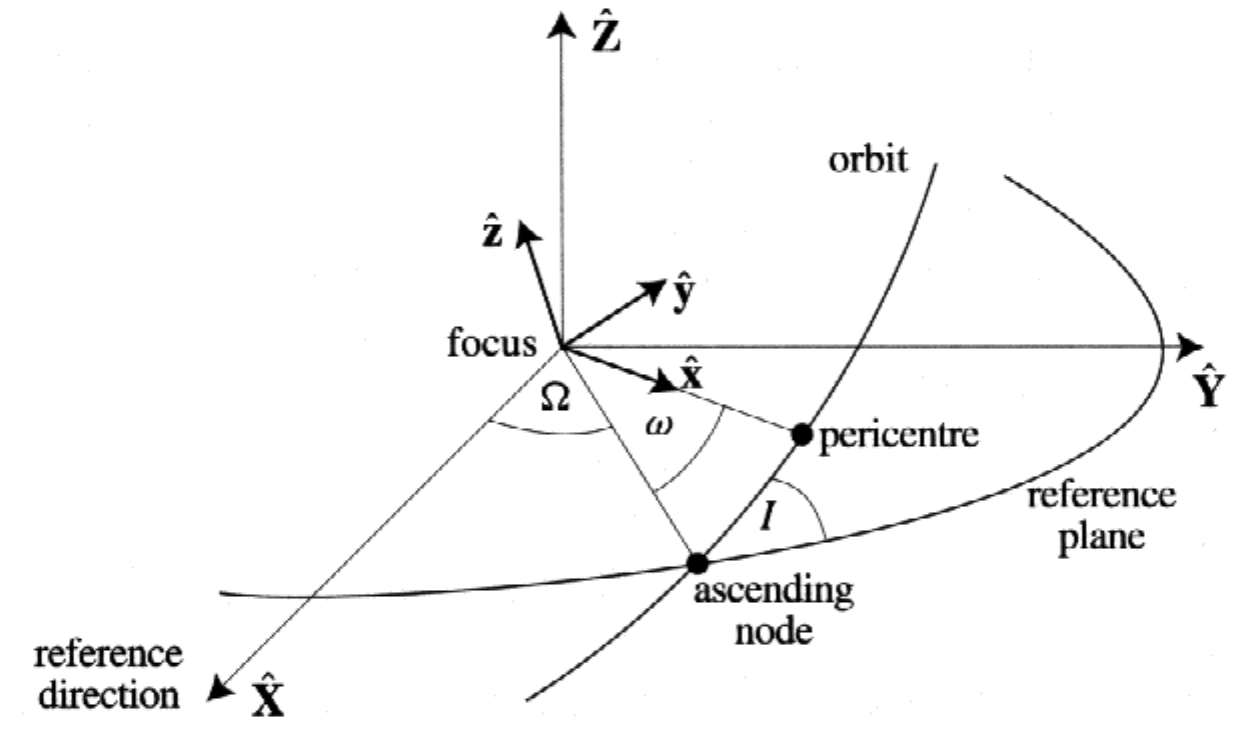
\includegraphics[width=0.8\linewidth]{gfx/3d_orbit.png}
\caption{A keplerian orbit in 3D space.}
\label{fig:3d_orbit}
\end{figure}
\Cref{fig:3d_orbit} shows the orbit in 3D cartesian coordinate system,
the reference plane is taken to be the $X-Y$ plane. The orbital
ellipse intersects the reference plane in two point. In order to define
its orientation relative to fixed axes we have to choose one. Independent
on wheater the orbiting body is moving around the ellipse in a clockwise
or counter-clockwise direction, the body will pass through the reference
plane \emph{from below} (where below is the $-Z$ direction)
at one of the two points. We call this point the \emph{ascending node}
and choose it as a reference. The angle from the ascending node to the
$X$ axis is then called the \emph{longitude of the ascending node} and
is denoted by $\Omega$. The angle between the plane of the ellipse and
the reference plane is called the \emph{inclination} of the orbit and
is defined in the range $0\leq I\leg \pi$.
Thus, we have completely described the orbit in 3D space. However, it is useful to 
define another angle $\pomega$ called the \emph{longitude of pericentre.} 
$\pomega$ is not really a true angle since it is defined as a sum of 
angles in two seperate planes. When the inclination is zero (the orbit
is co-planar with the reference plane) $\pomega=\omega$. 

It can be shown that each there is a one-to-one correspondance between 
a set of cartesian positions and velocities $(x,y,z,v_x,v_y,v_z)$ 
of a given massive particle and an \emph{instantaneous} Keplerian orbit 
defined by $(a,e,I,\Omega,\omega,f)$ with respect to another massive
particle. This why it is still usefull to talk about orbits even
when we are dealing with a system of multiple bodies. Altough those
bodies won't stay on a fixed Keplerian orbit for all time, at any given
time we can still define an instantaneous Keplerian orbit.

Most bodies in stable systems change their orbital elements slowly
when exchanging energy and angular momentum with other bodies, thus
it is often more useful to use the orbital elements as a set of coordinates
instead of the cartesian coordinates.

\section{A brief review of Hamiltonian mechanics}
\label{sec:hamiltonian_mechanics}
\subsection{Hamilton's equations}
\label{sub:Hamilton's equations}
The two--body prolem could have been solved equally well using a different
formulation of mechanics called \emph{Hamiltonian mechanics}. Hamiltonian
mechanics is equivalent to Newtonian mechanics but is often more suitable
for certain types of problems and the concept of a Hamiltonian function
is a lot more general than Newton's second law of mechanics.

In Newtonian mechanics the full description of a dynamical system 
consisting of N particles is 
obtained by solving a system of second order differential equations
of the form
\begin{equation}
    \dot{\vect{p}}_i=\vect{F}_i
\end{equation}
where $\dot{\vect{p}}_i=m_i\dot{\vect{r}}_i$ is the momentum of the
i-th particle, $m_i$ is its mass and $\vect{r}_i$ its position vector
relative to an origin of an inertial reference system. This 
constitutes a system of 3N second order differential equations for
the positions vectors $\vect{r}_i$. 

In the Hamiltonian formalism a dynamical system is described by 
a function of \emph{coordinates} $\vect{q}$ and \emph{momenta} 
$\vect{p}$ called the \emph{Hamiltonian} $\mathcal{H}(\vect{q},
\vect{p})$. The time evolution of these coordinates and momenta
$(\vect{q},\vect{p})$, collectively known as the \emph{phase space} 
is given by \emph{Hamilton's equations} 
\begin{equation}
    \dot{q}_i= \frac{\partial \mathcal{H}}{\partial p_i}\quad
    \dot{p}_i= \frac{\partial \mathcal{H}}{\partial q_i} 
\end{equation}
The solution of Hamilton's equations defines a trajectory in a 
6N dimensional phase space. The coordinate pair $(\vect{q},\vect{p})$
is said to be \emph{canonical} if the coordinates satisfy 
Hamilton's equations. The main advantage of the Hamiltonian
formalism compared to other formalisms of mechanics is the ability
to easily transform to different choices of $(\vect{q},\vect{p})$
as long as the new set of coordinates is also canonical. 


- be as clear as possible
- HM as one of several equivalent formulations, don't forget about
orders of diff. equations and Hamilton-Jacobi formulation
- don't forget that the key point of Hamilton's formulation is 
the equivalence of positions and momenta and the freedom to transform
the coordinates as we please as long as the transformation is canonical
- define a degree of freedom
- define what it means for a system to be integrable
- define generating functions
- maybe Liouville theorem

\section{The pendulum}
\label{sec:pendulum}
- follow either Mardling's non-hamiltonian approach or Allice's approach
- libration periods, driving forces...

\section{The three--body problem}
\label{sec:three_body}
- follow Mardling's nbody lectures, introduce mean mean--motion
resonances mathematically as slowly varying angles in  Fourier series
and physically, as repeated conjuctions of planets at the same location
in space.
- KAM theorem and invariant torii
- disturbing function
- secular and resonant interactions
- resonance widths (no plots for now)
- show that any Hamiltonian with a particular Harmonic can be reduced to
a single degree of freedom
- show that it is possible to systematically remove all other harmonics
by means of a canonical transformation
